\documentclass[a4paper,14pt]{article}

%%% Работа с русским языком
\usepackage{cmap}					% поиск в PDF
\usepackage{mathtext} 				% русские буквы в формулах
\usepackage[T2A]{fontenc}			% кодировка
\usepackage[utf8]{inputenc}			% кодировка исходного текста
\usepackage[english,russian]{babel}	% локализация и переносы
\usepackage{indentfirst}
\frenchspacing

\renewcommand{\epsilon}{\ensuremath{\varepsilon}}
\renewcommand{\phi}{\ensuremath{\varphi}}
\renewcommand{\kappa}{\ensuremath{\varkappa}}
\renewcommand{\le}{\ensuremath{\leqslant}}
\renewcommand{\leq}{\ensuremath{\leqslant}}
\renewcommand{\ge}{\ensuremath{\geqslant}}
\renewcommand{\geq}{\ensuremath{\geqslant}}
\renewcommand{\emptyset}{\varnothing}

\newcommand{\T}{^{\mathsf{T}}}
\newcommand{\uX}{\ensuremath{\underline{X}}}
\newcommand{\dH}{\mathbb{H}}
\newcommand{\dR}{\mathbb{R}}
\newcommand{\bz}{\mathbf{z}}
\renewcommand{\bf}{\mathbf{f}}
\newcommand{\bx}{\mathbf{x}}
\newcommand{\by}{\mathbf{y}}
\newcommand{\bv}{\mathbf{v}}
\newcommand{\bw}{\mathbf{w}}
\newcommand{\ba}{\mathbf{a}}
\newcommand{\bb}{\mathbf{b}}
\newcommand{\bp}{\mathbf{p}}
\newcommand{\bq}{\mathbf{q}}
\newcommand{\bt}{\mathbf{t}}
\newcommand{\bu}{\mathbf{u}}
\newcommand{\bT}{\mathbf{T}}
\newcommand{\bX}{\mathbf{X}}
\newcommand{\bZ}{\mathbf{Z}}
\newcommand{\bS}{\mathbf{S}}
\newcommand{\bH}{\mathbf{H}}
\newcommand{\bW}{\mathbf{W}}
\newcommand{\bY}{\mathbf{Y}}
\newcommand{\bU}{\mathbf{U}}
\newcommand{\bQ}{\mathbf{Q}}
\newcommand{\bP}{\mathbf{P}}
\newcommand{\bA}{\mathbf{A}}
\newcommand{\bB}{\mathbf{B}}
\newcommand{\bC}{\mathbf{C}}
\newcommand{\bE}{\mathbf{E}}


%%% Дополнительная работа с математикой
\usepackage{amsmath,amsfonts,amssymb,amsthm,mathtools} % AMS
\usepackage{icomma} % "Умная" запятая: $0,2$ --- число, $0, 2$ --- перечисление

%% Номера формул
%\mathtoolsset{showonlyrefs=true} % Показывать номера только у тех формул, на которые есть \eqref{} в тексте.
%\usepackage{leqno} % Нумереация формул слева

%% Свои команды
\DeclareMathOperator{\sgn}{\mathop{sgn}}

%% Перенос знаков в формулах (по Львовскому)
\newcommand*{\hm}[1]{#1\nobreak\discretionary{}
	{\hbox{$\mathsurround=0pt #1$}}{}}

%%% Работа с картинками
\usepackage{graphicx}  % Для вставки рисунков
\setlength\fboxsep{3pt} % Отступ рамки \fbox{} от рисунка
\setlength\fboxrule{1pt} % Толщина линий рамки \fbox{}
\usepackage{wrapfig} % Обтекание рисунков текстом

%%% Работа с таблицами
\usepackage{array,tabularx,tabulary,booktabs} % Дополнительная работа с таблицами
\usepackage{longtable}  % Длинные таблицы
\usepackage{multirow} % Слияние строк в таблице

%%% Теоремы
\theoremstyle{plain} % Это стиль по умолчанию, его можно не переопределять.
\newtheorem{theorem}{Теорема}[section]
\newtheorem{proposition}[theorem]{Утверждение}

\theoremstyle{definition} % "Определение"
\newtheorem{corollary}{Следствие}[theorem]
\newtheorem{problem}{Задача}[section]

\theoremstyle{remark} % "Примечание"
\newtheorem*{nonum}{Решение}

%%% Программирование
\usepackage{etoolbox} % логические операторы

%%% Страница
\usepackage{extsizes} % Возможность сделать 14-й шрифт
\usepackage{geometry} % Простой способ задавать поля
\geometry{top=25mm}
\geometry{bottom=35mm}
\geometry{left=35mm}
\geometry{right=20mm}
%
%\usepackage{fancyhdr} % Колонтитулы
% 	\pagestyle{fancy}
%\renewcommand{\headrulewidth}{0pt}  % Толщина линейки, отчеркивающей верхний колонтитул
% 	\lfoot{Нижний левый}
% 	\rfoot{Нижний правый}
% 	\rhead{Верхний правый}
% 	\chead{Верхний в центре}
% 	\lhead{Верхний левый}
%	\cfoot{Нижний в центре} % По умолчанию здесь номер страницы

\usepackage{setspace} % Интерлиньяж
%\onehalfspacing % Интерлиньяж 1.5
%\doublespacing % Интерлиньяж 2
%\singlespacing % Интерлиньяж 1

\usepackage{lastpage} % Узнать, сколько всего страниц в документе.

\usepackage{soul} % Модификаторы начертания

\usepackage{hyperref}
\usepackage[usenames,dvipsnames,svgnames,table,rgb]{xcolor}
\hypersetup{				% Гиперссылки
	unicode=true,           % русские буквы в раздела PDF
	pdftitle={Заголовок},   % Заголовок
	pdfauthor={Автор},      % Автор
	pdfsubject={Тема},      % Тема
	pdfcreator={Создатель}, % Создатель
	pdfproducer={Производитель}, % Производитель
	pdfkeywords={keyword1} {key2} {key3}, % Ключевые слова
	colorlinks=true,       	% false: ссылки в рамках; true: цветные ссылки
	linkcolor=red,          % внутренние ссылки
	citecolor=black,        % на библиографию
	filecolor=magenta,      % на файлы
	urlcolor=cyan           % на URL
}

\usepackage{csquotes} % Еще инструменты для ссылок

%\usepackage[style=authoryear,maxcitenames=2,backend=biber,sorting=nty]{biblatex}

\usepackage{multicol} % Несколько колонок

\usepackage{tikz} % Работа с графикой
\usepackage{pgfplots}
\usepackage{pgfplotstable}


\author{Владимиров Эдуард, группа Б05-928}
\title{\textbf{Отчёт о лабораторной работе №3}}
\date{\today}

\graphicspath{{./images/}}

\begin{document}
	\maketitle
	
	\section{Введение}
	Дано видео движения двухуровневый маятника в качестве исходного временного ряда и два временных ряда, которые соответствуют значениям углов, в качестве целевого временного ряда. 
	Необходимо, используя элемент фазового пространства, предсказать значения углов.  
	
	Весь код расположен по \href{https://colab.research.google.com/drive/1IIDZnvOCLYjBrD2ZFDvN9OzSxRKVDZBv?usp=share_link}{ссылке}
	
	\section{Постановка задачи}
	Введём обозначения:  
	
	$\uX \in \dR^{N \times I \times J}$ ~-- временной ряд кадров: число кадров $\cdot$ размеры изображения
	
	$Y \in \dR^{N \times 2}$ ~-- временной ряд звуков
	
	$T \in \mathbb{N}$ ~--- размерность траекторного пространства
	
	$\bX \in \dH_X \subset \mathbb{R}^{(N-T+1) \times T \times I \times J}$ ~--- траекторная матрица кадров и пространство траекторий
	
	$\bY \in \dH_Y \subset \mathbb{R}^{(N-T+1) \times T \times 2}$ ~--- траекторная матрица углов и пространство траекторий 
	
	
	$\bf: \dH_X \rightarrow \dH_Y$ ~--- предсказательная модель, полученная из HOPLS
	
	О том, как выглядит эта модель, будет сказано ниже.
	
	$\widehat{\bY} = \bf(\bX)$ ~--- предсказания модели
	
	$Q\left( \widehat{\bY}, \bY \right) = 1 - \dfrac{|| \widehat{\bY} - \bY||_F^2}{|| \bY ||_F^2}$ ~--- критерий качества модели
	
	\subsection{HOPLS}
	Для начала вспомним, как работает обычный PLS.  
	Для ранее нормированных по столбцам матриц $\bX$ и $\bY$ и числа компонент $K$ алгоритм работает следующим образом. 
	Положим $\bX_1 = \bX, \: \bY_1 = \bY$. 
	Далее для каждого $k \in [1, K]$:
	\begin{enumerate}
		\item вычисляем $\ba_k \in \dR^d$ и $\bb_k \in \dR^s$, первые левые и правые сингулярные вектора матрицы $\bX_k^T \bY_k$; из определения следует, что $(\ba_k, \bb_k) = \underset{\ba, \bb}{\text{argmax}} \text{ Cov} (\bX_k \ba, \bY_k \bb)$.
		\item проецируем матрицы $\bX_k$ и $\bY_k$ на сингулярные вектора: $\bt_k = \bX_k \ba_k, \; \bu_k = \bY_k \bb_k$.
		\item регрессируем матрицу $\bX_k$ по вектору $\bt_k$, то есть находим вектор $\bp_k$ такой, что матрица $\bt_k \bp_k\T$ является наилучшим одноранговым приближением матрицы $\bX_k$ по норме Фробениуса; делаем то же самое с матрицей $\bY_k$ и вектором $\bu_k$ и получаем вектор $\bq_k$.
		\item вычитаем из матрицы $\bX_k$ её одноранговое приближение из предыдущего шага, обозначим эту матрицу $\bX_{k+1}$; аналогичным образом получаем матрицу $\bY_{k+1}$.
	\end{enumerate}

	Метод HOPLS является расширением метода PLS на тензоры: вместо SVD-разложения произведения двух матриц ~--- HOOI-разложение тензорно-скалярного произведения двух тензоров и~т.д. 

	\begin{figure}[bhtp]
		\centering
		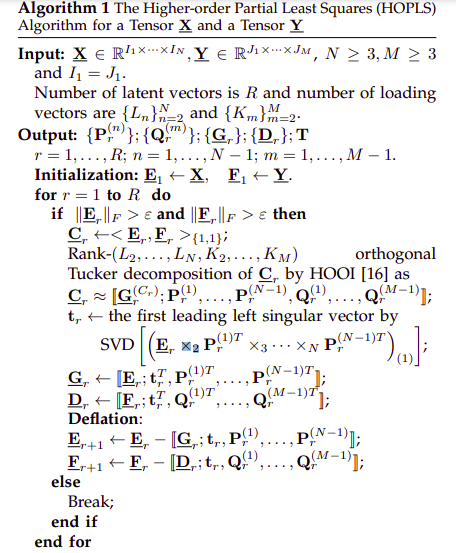
\includegraphics[width=0.8\linewidth]{hopls_algo.png}
		\caption{Полное описание алгоритма HOPLS}
	\end{figure}

	\begin{figure}[bhtp]
		\centering
		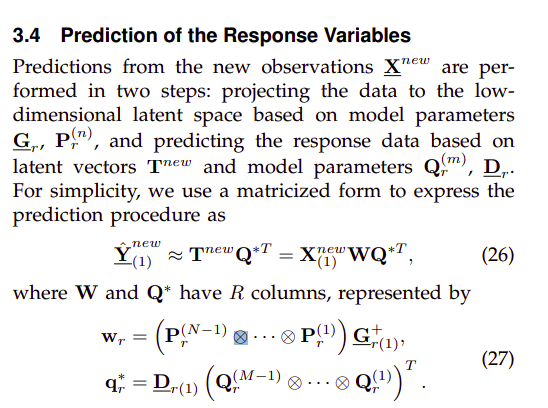
\includegraphics[width=0.8\linewidth]{hopls_prediction_model.png}
		\caption{Предсказательная модель $\bf$, полученная из HOPLS}
	\end{figure}

	\subsection{Двухуровневый маятник}
	\begin{figure}[bhtp]
		\centering
		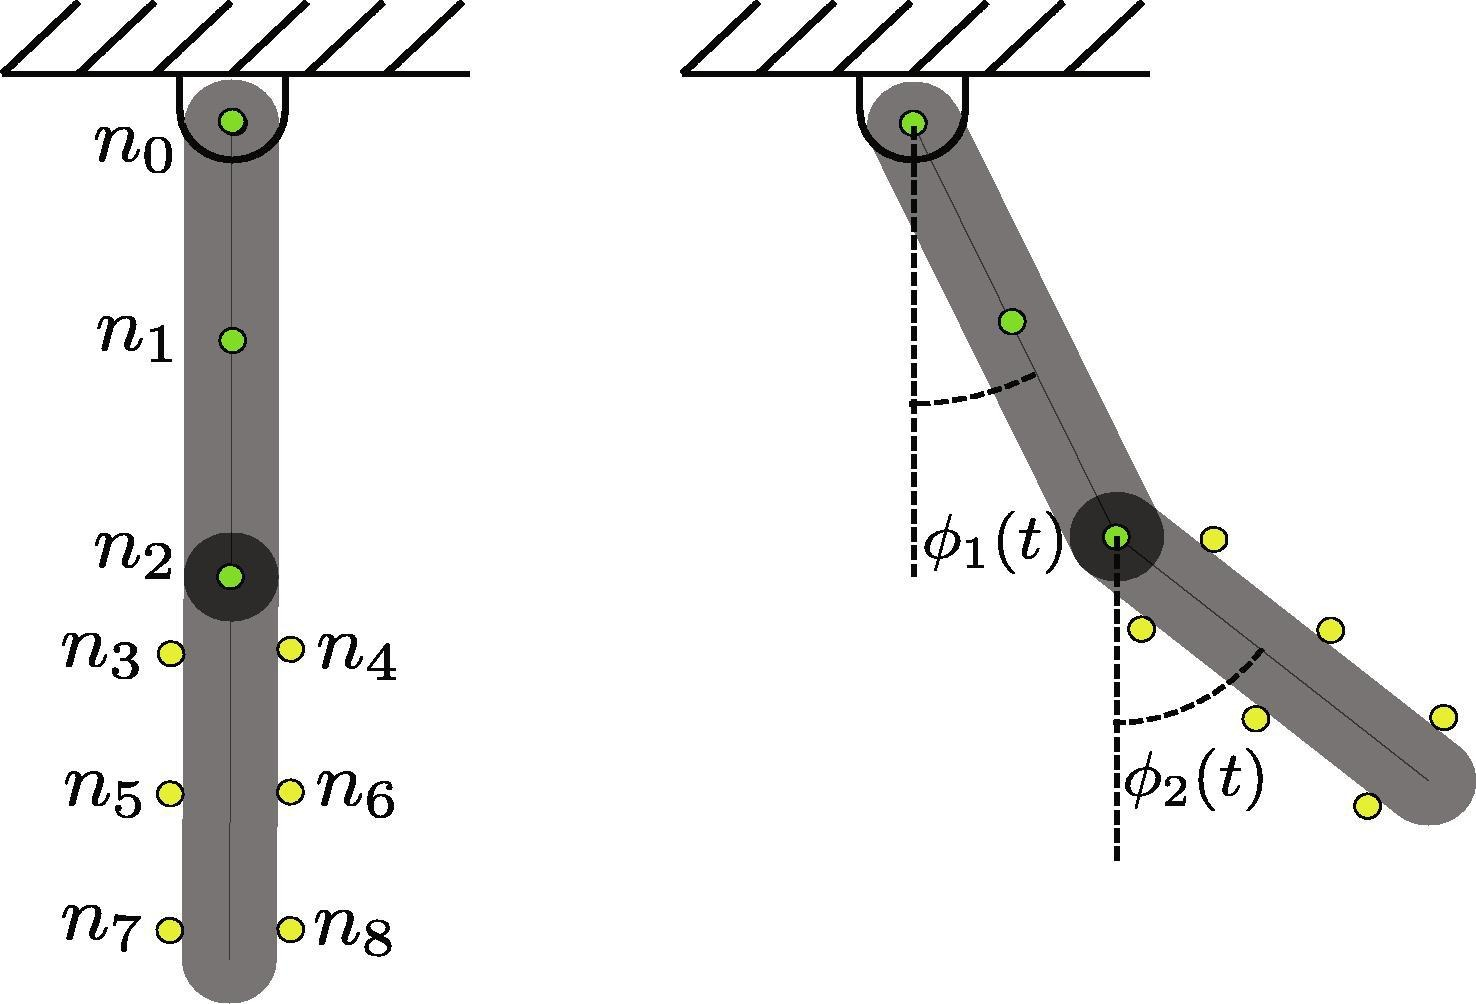
\includegraphics[width=0.9\linewidth]{complete_pendulum.jpg}
		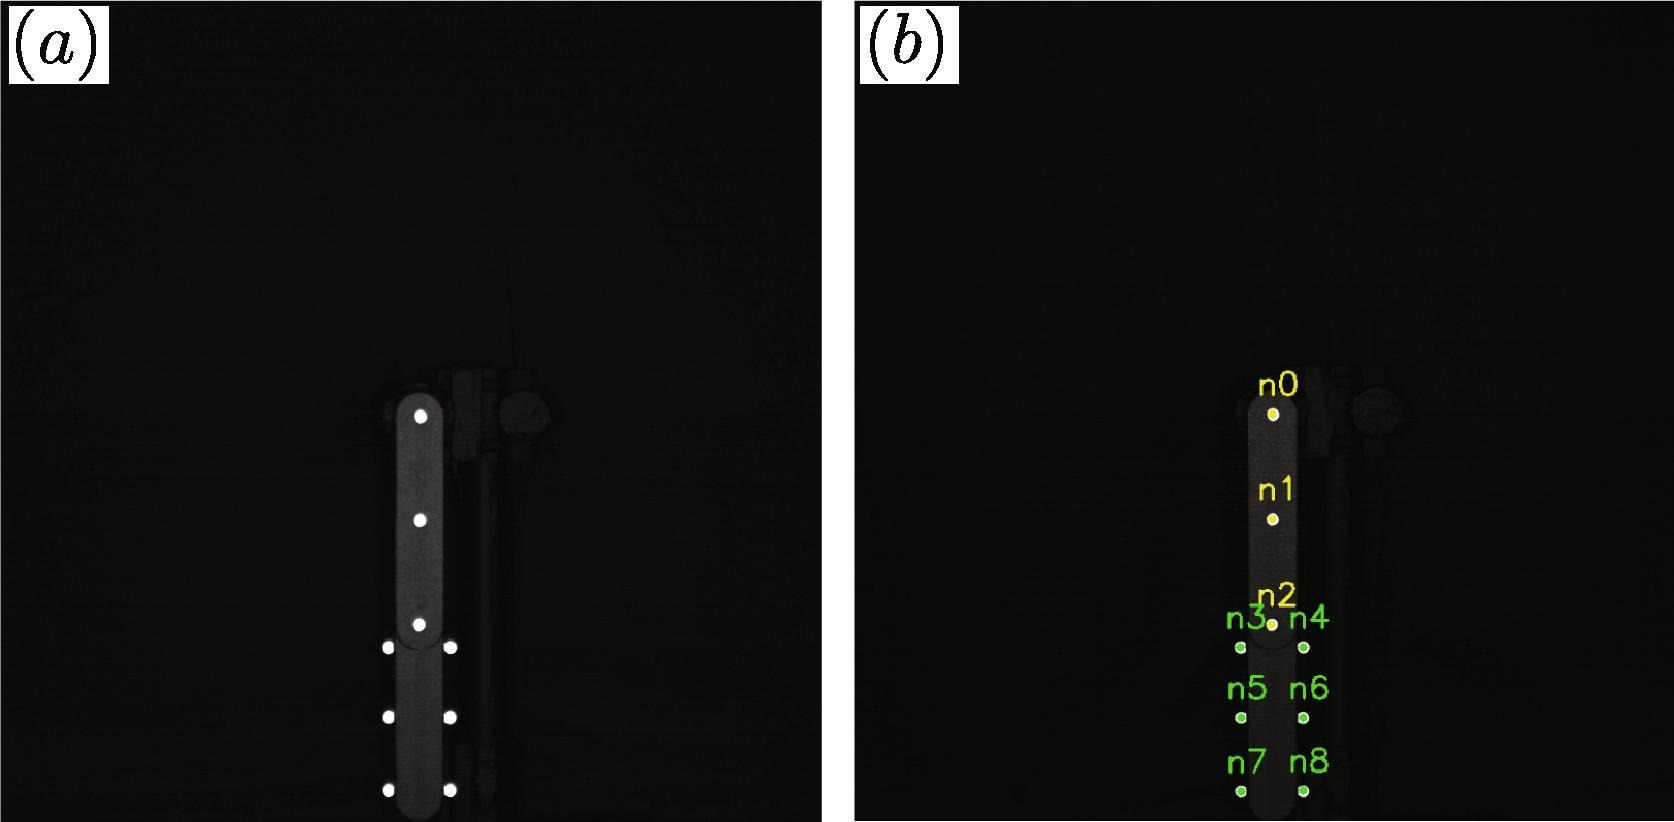
\includegraphics[width=0.9\linewidth]{double_pendulum}
		\caption{Внешний вид маятника}
	\end{figure}

	\section{Вычислительный эксперимент}
	Было взято видео движения маятника с разрешением $176 \times 240$, частотой 30 кадров в секунду и длительностью $\approx$6 минут.
	Общее число кадров равно 10802.  
	Отдельно стоит подчеркнуть, что видео снималось в замедленном режиме: 1 секунде реального времени соответствует 500 видео кадров, то есть частота составляет 500 Гц.  
	
	Затем для экономии памяти частота видеоряда уменьшается в 3 раза: с 500 Гц до 166.67 Гц, и сам видеоряд обрезается до 1500 кадров.  
	Для тестовой выборки взяты следующие 300 кадров.
	
	Размерность траекторного пространства равна 3.
	
	Далее применяется HOPLS со следующими гиперпараметрами: число компонент равняется $30$, размер core tensor-а ~--- $48 \times 48$. 
	Результаты модели показаны на графиках \ref{fig:metric_vs_components}, \ref{fig:train_and_test}.
	
	Из приведённых графиков можно заключить следующее:
	\begin{enumerate}
		\item Качество предсказания растёт с увеличением числа компонент
		\item HOPLS неплохо предсказывает значения углов на обучающей выборке, но на тестовой ведёт себя как константа. Предполагается, что это связано с наличием нелинейности в данных и с тем, что следующие значения целевой переменной сильно зависят от предыдущих. Её можно уменьшить, если вместо кумулятивных значений углов предсказывать обычные.
	\end{enumerate}

	Результаты поиска по сетке для обучающей выборки приведены в таблице \ref{tbl:grid_search_metrics}
	
	\begin{table}[]
		\begin{tabular}{lr|lll|lll|}
			\cline{3-8}
			& \multicolumn{1}{l|}{} & \multicolumn{3}{c|}{$\mathbf{\varphi_0}$} & \multicolumn{3}{c|}{$\mathbf{\varphi_1}$} \\ \cline{2-8} 
			\multicolumn{1}{l|}{} & \multicolumn{1}{l|}{\textbf{Kernel \textbackslash R}} & \multicolumn{1}{c|}{16} & \multicolumn{1}{c|}{32} & \multicolumn{1}{c|}{48} & \multicolumn{1}{c|}{16} & \multicolumn{1}{c|}{32} & \multicolumn{1}{c|}{48} \\ \hline
			\multicolumn{1}{|l|}{\multirow{3}{*}{\textbf{MSE}}} & 16 & \multicolumn{1}{r|}{8050} & \multicolumn{1}{l|}{6025} & \textbf{5855} & \multicolumn{1}{l|}{31309} & \multicolumn{1}{l|}{20308} & 19915 \\ \cline{2-8} 
			\multicolumn{1}{|l|}{} & 32 & \multicolumn{1}{r|}{7645} & \multicolumn{1}{l|}{8774} & 8774 & \multicolumn{1}{l|}{34576} & \multicolumn{1}{l|}{32797} & 32794 \\ \cline{2-8} 
			\multicolumn{1}{|l|}{} & 48 & \multicolumn{1}{l|}{8623} & \multicolumn{1}{l|}{7203} & 7055 & \multicolumn{1}{l|}{40114} & \multicolumn{1}{l|}{24345} & \textbf{19883} \\ \hline
			\multicolumn{1}{|l|}{\multirow{3}{*}{\textbf{MAE}}} & 16 & \multicolumn{1}{l|}{63.4} & \multicolumn{1}{l|}{\textbf{55.3}} & 58.2 & \multicolumn{1}{l|}{149.6} & \multicolumn{1}{l|}{104.6} & 101.2 \\ \cline{2-8} 
			\multicolumn{1}{|l|}{} & 32 & \multicolumn{1}{l|}{64.9} & \multicolumn{1}{l|}{77.1} & 77.1 & \multicolumn{1}{l|}{152.9} & \multicolumn{1}{l|}{145.6} & 145.6 \\ \cline{2-8} 
			\multicolumn{1}{|l|}{} & 48 & \multicolumn{1}{l|}{70.6} & \multicolumn{1}{l|}{61.9} & 63.2 & \multicolumn{1}{l|}{152.7} & \multicolumn{1}{l|}{116.0} & \textbf{104.9} \\ \hline
			\multicolumn{1}{|l|}{\multirow{3}{*}{$\mathbf{R^2}$}} & 16 & \multicolumn{1}{l|}{0.640} & \multicolumn{1}{l|}{0.730} & \textbf{0.738} & \multicolumn{1}{l|}{0.750} & \multicolumn{1}{l|}{0.837} & 0.841 \\ \cline{2-8} 
			\multicolumn{1}{|l|}{} & 32 & \multicolumn{1}{l|}{0.658} & \multicolumn{1}{l|}{0.607} & 0.607 & \multicolumn{1}{l|}{0.723} & \multicolumn{1}{l|}{0.738} & 0.738 \\ \cline{2-8} 
			\multicolumn{1}{|l|}{} & 48 & \multicolumn{1}{l|}{0.615} & \multicolumn{1}{l|}{0.678} & 0.684 & \multicolumn{1}{l|}{0.679} & \multicolumn{1}{l|}{0.805} & \textbf{0.841} \\ \hline
		\end{tabular}
		\label{tbl:grid_search_metrics}
		\caption{Метрики качества (MSE, MAE, $R^2$) модели предсказания кумулятивных углов маятника $\varphi_0, \, \varphi_1$ для разного числа компонент (R) и размера core tensor-а (Kernel)}
	\end{table}

	Также сравнены значения предсказаний кумулятивного и азимутного углов маятника, результаты приведены в таблице \ref{tbl:cum_vs_avi} и графике \ref{fig:azi_train_and_test}.

	\begin{figure}[bhtp]
		\centering
		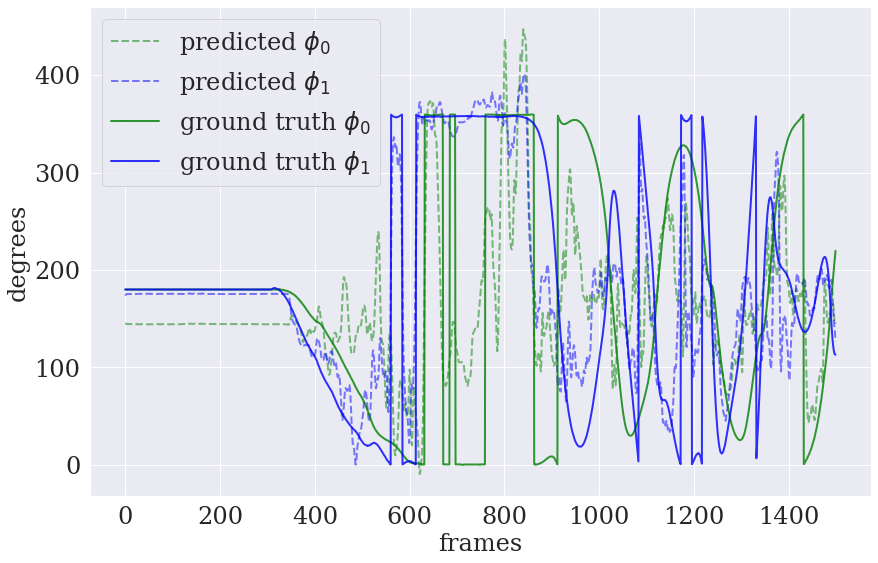
\includegraphics[width=0.7\linewidth]{train_azi_example}
		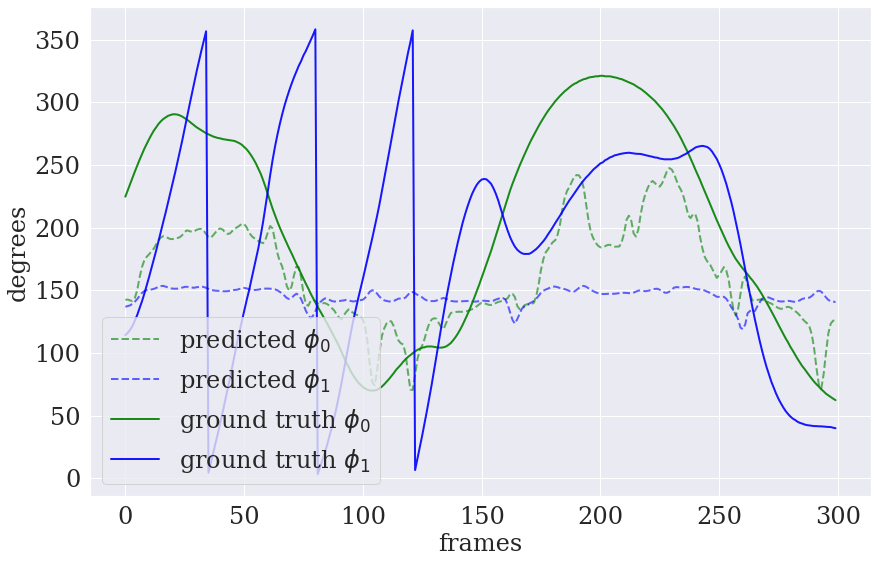
\includegraphics[width=0.7\linewidth]{test_azi_example}
		\caption{Результаты предсказания азимута угла на обучающей и тестовой выборках}
		\label{fig:azi_train_and_test}
	\end{figure}

	\begin{table}[]
		\begin{tabular}{l|cc|cc|}
			\cline{2-5}
			& \multicolumn{2}{c|}{\textbf{Cum}} & \multicolumn{2}{c|}{\textbf{Azi}} \\ \hline
			\multicolumn{1}{|l|}{\textbf{Metric \textbackslash Angle}} & \multicolumn{1}{l|}{$\mathbf{\varphi_0}$} & \multicolumn{1}{l|}{$\mathbf{\varphi_1}$} & \multicolumn{1}{l|}{$\mathbf{\varphi_0}$} & \multicolumn{1}{l|}{$\mathbf{\varphi_1}$} \\ \hline
			\multicolumn{1}{|l|}{\textbf{MSE}} & \multicolumn{1}{c|}{\textbf{7541}} & 27800 & \multicolumn{1}{c|}{7951} & \textbf{3708} \\ \hline
			\multicolumn{1}{|l|}{\textbf{MAE}} & \multicolumn{1}{c|}{\textbf{63.9}} & 120.6 & \multicolumn{1}{c|}{70.6} & \textbf{39.4} \\ \hline
			\multicolumn{1}{|l|}{$\mathbf{R^2}$} & \multicolumn{1}{c|}{\textbf{0.662}} & \textbf{0.778} & \multicolumn{1}{c|}{0.442} & 0.723 \\ \hline
		\end{tabular}
		\label{tbl:cum_vs_avi}
		\caption{Метрики качества (MSE, MAE, $R^2$) модели предсказания кумулятивного (Cum) и азимутного (Azi) углов}
	\end{table}
	
	\begin{figure}[bhtp]
		\centering
		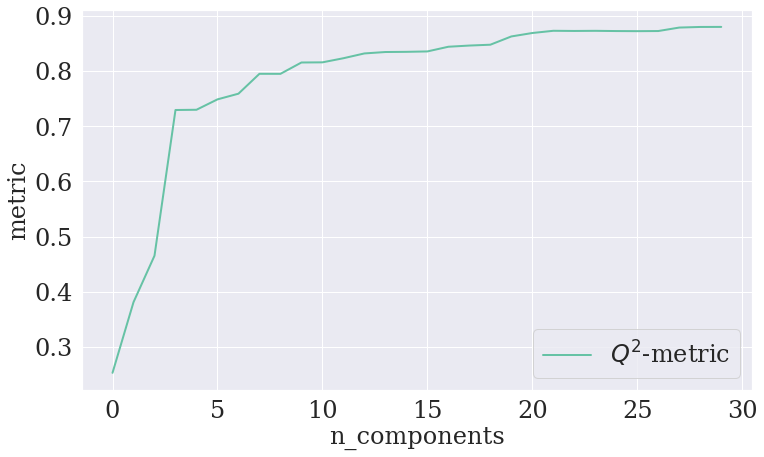
\includegraphics[width=0.8\linewidth]{metric-vs-components}
		\caption{Зависимость качества предсказания модели от числа компонент}
		\label{fig:metric_vs_components}
	\end{figure}

	\begin{figure}[bhtp]
		\centering
		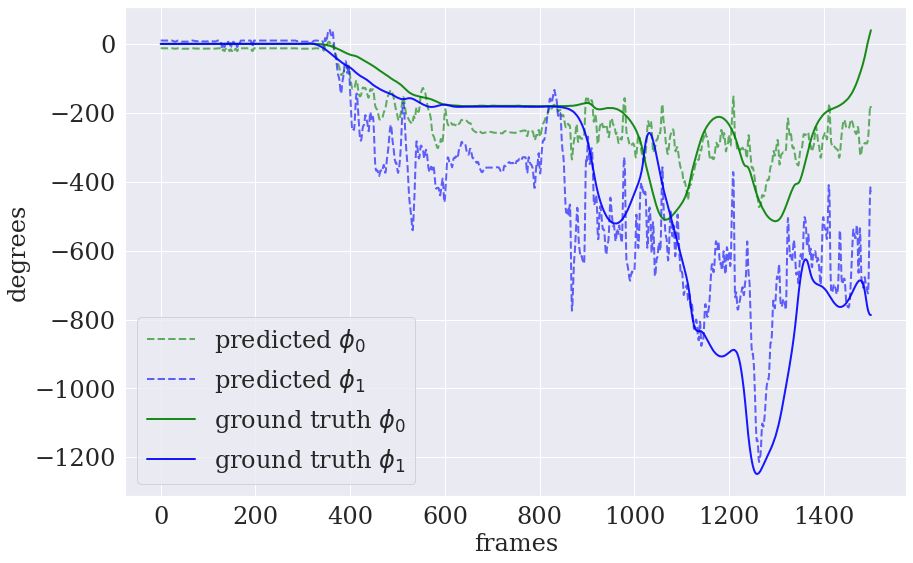
\includegraphics[width=0.7\linewidth]{train_example}
		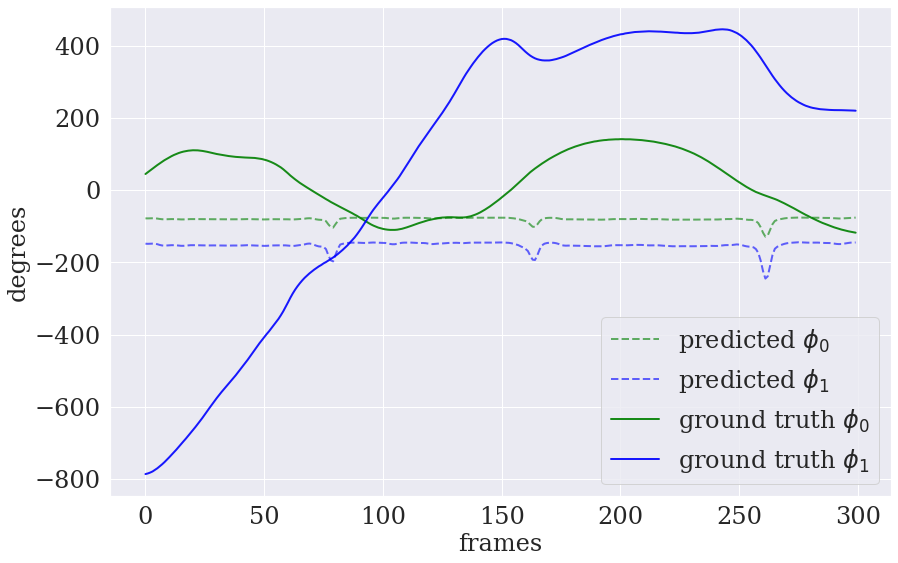
\includegraphics[width=0.7\linewidth]{test_example}
		\caption{Результаты предсказания на обучающей и тестовой выборках}
		\label{fig:train_and_test}
	\end{figure}

	\section{Литература}
	\begin{enumerate}
		\item Статья про HOPLS: \href{https://ieeexplore.ieee.org/stamp/stamp.jsp?arnumber=6365194}{ссылка}  
		\item Данные двухуровневого маятника: \href{https://www.sciencedirect.com/science/article/pii/S246806722030047X}{ссылка}
	\end{enumerate}
\end{document}
